\documentclass[12pt]{article}
\usepackage[margin = 1in]{geometry}
\usepackage[USenglish]{babel}
\usepackage{natbib}
\usepackage{graphicx}
\usepackage{fancyhdr}
\usepackage{setspace}
\usepackage{amsmath}
\usepackage{lscape}
\usepackage{dcolumn}
\usepackage{xcolor}
\usepackage{longtable}
\usepackage{tabularx}
\usepackage{booktabs}
\usepackage{arydshln}
\usepackage{dcolumn}
\usepackage[colorlinks=true,citecolor=red!50!black,urlcolor=blue!50!black,linkcolor=red!50!black]{hyperref}

\author{Patrick W. Kraft\footnote{Ph.D. Candidate, Stony Brook University, \href{mailto:patrick.kraft@stonybrook.edu}{patrick.kraft@stonybrook.edu}.
}}
\date{today}

\title{Looking for Answers\\
\large{A Naive Approach for Measuring Political Sophistication}\footnote{Previous versions of this manuscript have been presented at Polmeth 2016, MPSA 2017, EPSA 2017, and ISPP 2017.
The manuscript and code are available on GitHub: \url{https://github.com/pwkraft/knowledge}.
% I thank Jennifer Jerit, Jason Barabas (?), Yanna Krupnikov, Stanley Feldman, C{'e}line Colombo, Fabrizio Gilardi, Bill Jacoby, especially Scott, Jenn, and Celine for sharing data!
}
}
\date{\today}

% sans serif font
\renewcommand{\familydefault}{\sfdefault}


\begin{document}
\maketitle
\doublespacing
\thispagestyle{empty}

\begin{center}
-- WORK IN PROGRESS -- \\
PLEASE DO NOT CITE OR REDISTRIBUTE WITHOUT PERMISSION
\end{center} 

\hfill
\begin{abstract}\singlespacing
This paper proposes a simple but powerful framework to assess political sophistication in verbatim responses to open-ended survey questions. The measure aims to capture the complexity of individual attitude expressions by examining their relative length, topic diversity, and opinionation. I validate the approach by comparing it to conventional political knowledge metrics in multiple studies using different batteries of open-ended items. The paper proceeds to illustrate how text-based sophistication helps refine important previous insights from the literature, for example regarding the oft-cited gender gap in political knowledge.
% This is just a placholder abstract for now, needs some serious revisions.
% QUESTION: measure can be based on different sets of items

%\vspace{\baselineskip}
%\noindent \textbf{Keywords:} political sophistication, gender gap, measurement, open-ended responses, text analysis \\

\end{abstract}
\hfill
\newpage\setcounter{page}{1}


% REVISE: mention data sources earlier in the manuscript?
% REPLACE: "recall" instead of "factual" knowledge questions

Alarmingly high levels of voter ignorance have been one of the major recurring themes in public opinion research. Not too long ago, for example, \citet{bartels2005homer} attributed public support for the Bush administration's 2001 and 2003 tax cuts to a substantial lack of political information among voters \citep[but see][]{lupia2007were,bartels2007homer}. Similarly, Delli Carpini and Keeter's \citeyearpar{carpini1996americans} seminal book on political knowledge warned that widespread ignorance might jeopardize equal representation of citizens. Early influential scholars such as \citet{converse1964nature} also emphasized that large parts of the public lack a sufficient understanding of abstract ideological concepts and do not hold stable issue positions. Indeed, the finding that citizens know little about politics seems to go as far back in history as the systematic study of public opinion itself.

Yet, not everyone agrees with this pessimistic assessment. Instead, there has been a lively debate about how to accurately assess political knowledge in the first place \citep[e.g.][]{mondak2000reconsidering,mondak2001asked,sturgis2008experiment,debell2013harder,pietryka2013analysis}. Most analyses rely on standard item batteries that assess individuals' factual knowledge about political institutions and officeholders \citep[e.g.,][]{carpini1996americans}. However, recent research points to important distinctions in types of political knowledge that have previously been disregarded \citep{barabas2014question}. Furthermore, scholars argue that recall-based measures of political knowledge do not necessarily capture how people structure their attitudes and beliefs \citep[e.g.,][]{luskin1987measuring} and may not be theoretically relevant for the development of informed preferences \citep[e.g.,][]{lupia2006elitism,gilens2001political}.

% JENN: cut this para, cite gilens
%The last point raises a fundamental question about the type of knowledge that is actually necessary for outcomes we view as desirable \citep[see also][]{lupia2015uninformed}: Do citizens really need to know specific details about US political institutions in order to successfully engage in politics? For example, precise knowledge of the official term lengths of U.S. Senators can hardly be viewed as necessary to cast an informed vote between two candidates running for President. This is especially the case since voters can rely on heuristics \citep{lupia1994shortcuts} or procedural knowledge \citep{prior2008money} when forming political preferences. Factual knowledge as measured in many public opinion surveys may therefore not be an ideal indicator for citizens' competence to engage in politics.

% More direct/active language in this para:
This article develops alternative measure of political sophistication that aims to address this disconnect. Normative democratic theory suggests that voters should hold informed opinions about available candidates and relevant issues before casting a vote. Rather than relying on factual knowledge that is potentially unrelated to the task at hand, I examine how respondents discuss their political preferences and beliefs in their own words. For a given set of verbatim responses, the measure assesses political sophistication based on relative response lengths, diversity in topics raised by individuals, as well as their level of opinionation. The approach is therefore \textit{naive} in that it does not presuppose pieces of information as necessary for political competence but rather examines the respondents' justification of their preferences at face value. The goal is to assess whether political attitudes relevant to perform a specific task are expressed in a more elaborate manner---a question that is not directly discernible when examining off-the-shelf factual knowledge items. %The text-based measure is therefore conceptually closer to the degree of structure and constraint in political belief systems \citep[see for example][]{tetlock1983cognitive,luskin1987measuring}. 

% TODO: revise this section, predictor part comes out of nowhere
The proposed measure is validated across multiple data sets by comparing it to conventional factual knowledge scores as predictors of competences relevant to perform political tasks. While the measures share a considerable amount of variance, they are far from equivalent. Indeed, text-based sophistication is a stronger predictor of internal efficacy, political engagement, and turnout than most traditional measures. After validating the measurement approach, the paper illustrates how text-based sophistication can help refine previous insights in the literature by re-examining an oft-cited finding in empirical research---the gender gap in political knowledge. Contrary to previous research, I find no evidence for such a gap based on open-ended responses. While women might score lower than men on factual knowledge about political institutions and elites, there are no differences in the complexity of expressed political attitudes. More generally, the results suggest that developing valid measures of political sophistication based on open-ended responses can provide new opportunities to examine political knowledge across time and contexts. 


\section*{Factual Knowledge and Political Competence}
%\section*{Recalling Facts Does Not Imply (Political) Competence}
% 1: gender gap is a commom phenomenon in the literature
% 2: potential explanations based on measurement
% 3: broader issue: do we need political facts or structure of belief systems? competence?
% ADD: section on the role of competences etc.
% REVISE: all tests of political knowlege should follow based on the required competences

% A lot of political science research focuses on political knowledge, but that's not really what we should care about.
% - Druckman argument: Issue of representation, why common indicators of political knowledge are insufficient. What are the alternatives? Think of attitude formation!
% - Lupia argument: identify a task and the necessary competences. Criteria to select knowledge questions are often random, not guided by theory about necessary competences. Think about what people need to do, then think about how to assess whether they can do that.

% JENN: cut both paras, they are repetitive w/ opening... maybe use some of the citations?
%A common theme in public opinion research revolves around the question whether citizens fulfill the requirements necessary to hold their elected officials accountable. Pioneered by \citet{carpini1996americans} and others, much of this inquiry has focused on individual levels of factual knowledge about political institutions and officeholders \citep[see also][]{carpini1993measuring}. For example, \citet[21]{zaller1992nature} argued that testing factual information about politics provides the best available measure of political awareness, since it ``more directly than any of the alternative measures, capture[s] what has actually gotten into people’s minds.'' Studies in this area frequently attest that large parts of the public do not meet the standards determined by researchers. Quite contrary, the citizenry appears mostly disengaged, uninterested, and above all ill-informed about politics, which can ultimately result in unequal representation in the political system \citep[e.g.,][]{althaus1998information,kuklinski2000misinformation,gilens2001political}.

%However, this is not the only recurring theme in the literature related to citizens' level of information. Instead, there are frequent debates about the proper measurement of political knowledge. For example, \citet{krosnick2008problems} emphasized problems related to the coding rules of common recall items included in the American National Election Study, which fail to properly capture partial knowledge \citep[see also][]{gibson2009knowing,debell2013harder}. \citet{mondak2000reconsidering} raised additional concerns by showing that individual performance on political knowledge items is influenced by differential probabilities to engage in guessing \citep[see also][]{mondak2001developing,mondak2001asked,miller2008experimenting}. While the question of measurement using knowledge items is certainly an important debate with noteworthy recent contributions \citep[e.g.,][]{pietryka2013analysis}, there is a more fundamental theoretical issue related political sophistication that is frequently overlooked: \textit{What do citizens need to know in order to participate effectively in the democratic process?}

% THIS STILL NEEDS REVISIONS, especially the last part. maybe elaborate on barabas?
The most important task for citizens in a modern democracy is to vote for candidates who represent their interests and hold their elected officials accountable. Arguably, survey items measuring political knowledge should therefore cover information that is necessary and/or sufficient to perform this essential task. However, determining such a set of items proves to be extremely difficult (if not impossible), especially since there are systematic differences in types of knowledge \citep{barabas2014question} and survey questions typically cannot capture important aspects such as visual cues \citep{prior2014visual}. Conceptualizing political knowledge, \citet{barabas2014question} distinguished both, a temporal dimension (i.e., whether it is static or more contemporary) as well as a topical dimension (i.e., whether it is general or more policy-specific). Importantly, varying the types of questions on these dimensions leads to different conclusions regarding the nature and determinants of political knowledge. However, even within a given category, people may disagree about which facts are important due to inherent value differences \citep[c.f.,][]{lupia2015uninformed}. As such, even if we had strong theoretical reasons to focus on a certain set of questions according to the typology developed by \citet{barabas2014question} there would still be uncertainty about the specific set of facts deemed as necessary to perform a political task. Despite these difficulties, most empirical studies simply relied on a set of off-the-shelf knowledge questions that have been used in previous research rather than justifying their choices from a theoretical perspective. As \citet[219]{lupia2006elitism} explains, ``Most political knowledge questions are not derived from a replicable or transparent logic about how their answers bear on a voter's ability to make decisions of a particular quality.'' As such, information requested in conventional survey items often have no clear relevance to political participation. 

\citet{lupia2006elitism} argues that instead of focusing on potentially irrelevant factual knowledge, researchers should concentrate on heuristics that directly help citizens to make competent political decisions or focus only on knowledge relevant to a specific task \citep[see also][]{lupia1994shortcuts,lupia2015uninformed}. After all, there is no need for individuals to know all available facts, but only to possess the skills and resources to be able to \textit{find} the information required in a specific context \citep{prior2008money}. \citet{druckman2014pathologies} makes a similar argument in a recent review of research on public opinion and democratic responsiveness. Since there is no apparent consensus about the precise measurement of political knowledge and it is unclear what information is necessary in the first place, the author proposes to direct the attention away from individual levels of political information as a measure of ``quality opinion''. Instead, \citet[478, emphasis in the original]{druckman2014pathologies} advocates ``\textit{less} focus on the \textit{content/substance} of opinions (e.g., are they informed, constrained, based on strong frames, etc.?) and \textit{more} on the \textit{process} and specifically the \textit{motivation} that underlies the formation of those opinions.'' The framework proposed herein follows this line of reasoning in attempting to measure political sophistication based on expressed attitudes related to a specific political task.
% Make sure in the following discussion that it's clear that the measure focuses more on the structure and motivation as described by Druckman!


\section*{Opinion Formation and Attitude Expression}
%\section*{What do People Have to Say About the Issues?}
% ADD: issue of item choice, etc.
% ADD chapter reviewing approaches that focus on linguistic complexity, dictionaries capturing integrative complexity etc..

% Rather than using off-the-shelf item batteries to measure general knowledge, we can simply ask respondents to discuss their preferences in beliefs in a specific field of substantive interest and then go from there.
% Discuss colombo article here

Rather than trying to develop a new item battery that presupposes a set of facts as necessary for political competence---a task that is difficult to achieve---I propose to analyze how individuals discuss their attitudes and preferences related to a political task in their own words. Citizens have to engage in a lot of choices in democratic politics. For example, they can vote in local, state, or federal elections. Depending on the institutional setup, they may also directly decide on specific policies through referenda. In these contexts, we are often concerned whether citizens are able to make high quality decisions in accordance with their preferences. According to \citet{druckman2014pathologies}, scholars should concentrate on whether individuals are motivated to engage in accurate and objective processing when forming their opinions rather than trying to assess their level of factual knowledge. Importantly, a major approach to induce accuracy motivations discussed by \citet[478]{druckman2014pathologies} involves asking individuals to ``justify/provide reasons for one's opinions.'' Conversely, we may directly examine \textit{how} citizens justify their preferences in order to evaluate their level of sophistication in attitude expression. To the extent that respondents engage in accurate processing to form quality opinions, they should be able to discuss multiple considerations related to a political issue and show awareness of arguments for and against certain positions.

Such a perspective resembles influential theoretical accounts of political sophistication which focus on the \textit{structure} of belief systems rather than the content (or accuracy) of related considerations. In his seminal article, \citet{converse1964nature} emphasized the importance of the level of conceptualization as the main characteristic of sophistication rather than isolated pieces of factual information. Similarly, \citet{tetlock1983cognitive} used the term \textsl{integrative complexity} to describe the degree to which considerations related to an issue are interconnected. \citet{luskin1987measuring} also defined political sophistication based on the structure of individual belief systems, arguing that they can vary on three separate dimensions: (1) their \textsl{size} -- i.e. the number of cognitions, (2) their \textsl{range} -- i.e. the dispersion of cognition over categories, and (3) their \textsl{constraint} -- i.e. the extent to which cognitions are interconnected in a meaningful way. Political sophistication, in turn, is seen as the conjunction of these dimensions: ``A person is politically sophisticated to the extent to which his or her [political belief system] is large, wide-ranging, and highly constrained.'' \citep[860]{luskin1987measuring}. These differences in sophistication should be reflected in the way individuals describe, discuss, and justify their political beliefs.

\citet{colombo2016justifications} makes a similar argument when investigating the level of competence of Swiss citizens to vote in policy referenda. Examining data from thirty-four ballot decisions, the author analyzes how voters justify their individual decision in favor or against a certain policy in open-ended survey responses. More specifically, she proposes to ``consider the capacity to justify political decisions with policy-related arguments as a possible conceptualization of citizen competence in direct democracy'' \citep[3]{colombo2016justifications}. Levels of justification are thereby measured based on a manual coding of each answer's content, elaboration, and complexity. \citet{colombo2016justifications} finds that while Swiss citizens are indeed able to provide policy-related arguments to justify their decisions, their level of competence is influenced by the political context and individual resources.

Examining individual levels of justification in open-ended responses as a measure of political competence is not only applicable to referenda in direct democracies. It can also be implemented in diverse settings involving various types of political preferences. From a theoretical perspective, the same arguments regarding the structure of individual belief systems holds when examining different types of open-ended responses, for example when respondents discuss their attitudes toward candidates running for office. As such, in order to measure sophistication and competence related to a political task of interest, I propose to examine how individuals discuss and justify their related preferences in their own words instead of relying off-the-shelf knowledge items. However, manual coding of open-ended responses as employed by \citet{colombo2016justifications} is not always feasible in the context of large-scale surveys, since it can be very labor-intensive, requires a large amount of contextual knowledge, and -- depending on the country -- necessitates high levels of language proficiency.\footnote{The Swiss surveys in Colombo's \citeyearpar{colombo2016justifications} study were conducted in three different languages: German, French, and Italian.} While manual coding could therefore be seen as the gold standard, I now present a simple but powerful approach that relies on quantitative text-analysis methods and can be applied in multiple contexts and different languages.


%\section*{Factual Problems with Political Knowledge}
\section*{Measuring Text-Based Sophistication}
% 1: if we care about the structure of belief systems, how would they respond to open-ended items?
% 2: how are open-ended responses administered, potential issues
% describe dataset and open-ended responses
% describe measure for each dimension as well as composite measure of sophistication

% ADD: differentiate from manual coding of integrative complexity (labor intensive) and dictionary-based methods (focus on linguistic characteristics, which could easily conflate general eloquence)


How would a politically sophisticated person discuss his or her views compared to a less informed individual? Consider a survey where respondents are asked to describe their attitudes toward specific policies or candidates running for office in verbatim. In such a scenario, the structure of individual political belief systems (i.e., size, range, and constraint) should be reflected in their responses to a set of open-ended items. In the following, I discuss three different attributes of open-ended survey responses that should be indicative of individual political sophistication as described by \citet{luskin1987measuring} and others.

First of all, sophisticated individuals should be able to elaborate more on their political attitudes. If people possess a large, wide-ranging, and constrained belief system, they should be able to recall a large number of considerations related to political actors or issues. Verbatim responses of sophisticates can therefore be expected to have a greater overall \textbf{length}, which is measured as the logged word count for each individual over all prompts:
\begin{equation}
\text{length}_i = \dfrac{\log\left(\sum_{j=1}^J n_{ij}\right)}{\max\left[\log\left(\sum_{j=1}^J n_{ij}\right)\right]},
\end{equation}
where $n_{ij}$ is the number of words in the response of individual $i$ in response to question $j$. $J$ denotes the set of all open-ended probes. I use the logged count to normalize the distribution of responses and divide it by the maximal response length in the data such that the resulting measure ranges from 0 to 1.

However, sophisticated individuals should not only be able to talk about their attitudes at greater lengths. It is also important to consider the content of their respective answers. If a respondents holds more diverse cognitions towards political actors or policies, we should observe a wider range of topics addressed in their responses rather than a focus on single issues. As such, verbatim responses of political sophisticates should display a greater degree of \textbf{topic diversity}, which is conceptualized as the relative mean absolute difference in topic proportions:\footnote{Individual topic proportions are extracted from a structural topic model estimated using the \texttt{stm} package in R \citep{roberts2014structural}. Please refer to the appendix for more information on the topic model as well as the robustness for varying specifications. % The number of topics was selected using the algorithm of \citet{lee2014low} and the model was estimated via spectral initialization to address the issue of multi-modality \citep[see][for details]{roberts2014stm}. I use measures for age, education, party identification, as well as an interaction between education and party identification as covariates for topic prevalence. This variable selection is equivalent to the procedure model specification described in \citet{roberts2014structural. I estimated a total number of 72 topics. The results reported hereafter are robust for model specifications with fewer numbers of topics.
}
\begin{equation}
\text{topic diversity}_i = 1-\dfrac{\sum_{k_1=1}^K\sum_{k_2=1}^K |\theta_{ik_1} - \theta_{ik_2}|}{2K\sum_{k_1=1}^K \theta_{ik_1}},
\end{equation}
where $\theta_{ik}$ denotes the predicted proportion of topic $k$ in the collection of responses by individual $i$. The variable ranges from 0 (response focuses on single topic), to 1 (every topic has the same proportion). Mathematically, this conceptualization is equivalent to the Gini-coefficient, which measures the degree of inequality in income distributions (although the direction has been reversed such that a value of 1 implies a perfectly equal distribution).

Lastly, sophisticated individuals should hold opinions about each political actor or policy that they are asked to discuss. As such, shophisticates should be able to express their attitudes towards each open-ended probe in terms of both, approval or disapproval. Responses that reflect high levels of sophistication should therefore display a greater level of \textbf{opinionation}, which is measured as the relative mean absolute difference of relative response lengths for each open-ended response:
\begin{equation}
\text{opinionation}_i = 1-\dfrac{\sum_{j_1=1}^J\sum_{j_2=1}^J |p_{ij_1} - p_{ij_2}|}{2J\sum_{j_1=1}^J p_{ij_1}},
\end{equation}
where $p_{ij}=\tfrac{n_{ij}}{\sum_{j=1}^J n_{ij}}$ is the proportion of words in the response of individual $i$ to question $j$ relative to the overall size of the individuals' response. Again, the variable ranges from 0 (only one question was answered) to 1 (all questions were answered with the same word length per answer).

Together, the three measures form a composite metric of political sophistication by calculating their respective average for each respondent. Like each individual component, the resulting \textbf{text-based sophistication} score ranges from 0 to 1:
\begin{equation}
\text{text-based sophistication}_i = \tfrac{1}{3}(\text{length}_i + \text{topic diversity}_i + \text{opinionation}_i).
\end{equation}

Overall, a highly sophisticated individual can be expected to respond to a set of open-ended items by giving a more elaborate response that focuses on multiple considerations or topics and addresses his or her attitudes towards all relevant political actors or policies more or less equally.\footnote{Note that this approach differs from recent work on sophistication in political speeches \citep[e.g.,][]{spirling2016democratization} as it explicitly tries to capture complexity independent of pure linguistic style.}


% QUESTION: Validate measure before actual application? I think that would make sense

% QUESTION: think about other factors determined by political sophistication

% CONTINUE HERE

\section*{An Overview of Data Sources and Open Ended Items}

The text-based sophistication measure is validated using multiple surveys employing different sets of open-ended questions. Each data set and the respective items used to compute text-based sophistication are briefly described below. Please refer to the appendix for more detailed information on the data and methods, such as pre-processing the verbatim responses.


[ADD GERMAN GENERAL SOCIAL SURVEY DATA?]

\subsection*{American National Election Study 2012}

The main analyses are based on the 2012 American National Election Study (ANES), which consists of a representative survey of 5914 adults in the months before the 2012 US Presidential election. 2054 respondents participated in face-to-face interviews while the remaining 3860 filled out the survey online. For the purpose of the present analysis, I rely on the pooled dataset while controlling for differences in survey mode. The text-based sophistication measure is based on open-ended questions in which respondents were asked in the pre-election wave of the survey to list anything in particular that they like/dislike about the Democratic/Republican party as well as anything that might make them vote/not vote for either of the Presidential candidates. They were probed by the interviewer asking ``anything else?'' until the respondent answered ``no''. Overall, there are a total number of 8 open-ended responses where individuals described their beliefs and attitudes towards political actors. Individuals who did not respond to all of the open-ended items (417 individuals), or who responded in Spanish (228 individuals), were excluded from the analysis.\footnote{Please see Appendix A for descriptive information on the individual components of the text-based sophistication measure. % Verbatim responses were pre-processed using the Aspell spell-checking algorithm (\url{www.aspell.net}).
}

\subsection*{2015 Yougov Survey}

In order to replicate and extend the main analyses, I rely on a separate nationally representative survey employing an alternative set of open-ended responses. The data was collected by YouGov in December 2015 and contains responses of 1000 U.S. citizens.\footnote{See \citet{clifford2016cheating} for details on the study.} As part of this study, respondents were asked to describe their attitudes towards two prominent political issues that were discussed frequently in the media. First, they were asked in a closed format whether they favor or oppose stricter gun laws. Subsequently, they were asked to respond to the following two questions in verbatim:
\begin{itemize}
\item Still thinking about the question you just answered, what thoughts came to mind while you were answering that question? Please try to list everything that came to mind.
\item Thinking about the mass shootings that have occurred in the U.S. in the last few years, what factors do you think are responsible for the shootings?
\end{itemize}
Second, the respondents report on their attitudes towards the Affordable Care Act in a closed format and are then asked to elaborate in their own words by answering the following questions:
\begin{itemize}
\item Still thinking about the question you just answered, what thoughts came to mind while you were answering that question? Please try to list everything that came to mind.
\item For decades, experts have observed that the United States spends far more per person on health care than any other country. However, the U.S. falls behind on most measures of health care outcomes, such as life expectancy. What factors do you think are responsible for the state of our health care system?
\end{itemize}
Here, the text-based sophistication measure is computed based on the verbatim responses to the four preceding questions using the same procedures described above. Compared to the open-ended likes/dislikes items included in the 2012 ANES, the questions directly address considerations related to specific policy issues that were prominent in the political discourse at the time of the survey.\footnote{Please see Appendix B for descriptive information on the individual components of the text-based sophistication measure.}

% HOW MANY DID NOT RESPOND???



\subsection*{Swiss Referendum Data}

Lastly, I examine the data used in the analyses presented by \citet{colombo2016justifications} to compare text-based sophistication to manual coding of open-ended responses. The author compiled a data set from cross-sectional surveys that were conducted in Switzerland after national popular votes on multiple policy propositions. Within the surveys, respondents were asked to justify why they voted in favor or against a given proposition. \citet{colombo2016justifications} manually recoded the verbatim responses to measure individual \textit{levels of justification}, which combines dimensions of answer content, elaboration, and complexity.

The original surveys were conducted with 26,621 Swiss citizens after one of thirty-four policy votes that were held between 2008 and 2012. However, respondents were only asked to justify their decision in verbatim if they participated in the vote.

% QUESTION wording?
% NUMBER OF RESPONDENTS DROPPPED?



\section*{Comparing the Measures}


Before turning to the actual validation, I begin by directly comparing the text-based sophistication measure to alternative metrics of political knowledge in the 2012 ANES. The most common way to measure political knowledge in surveys is to ask a set of factual questions about political institutions. The ANES includes such a basic item battery, inquiring for example about the number of times an individual can be elected President of the United States, or how the current U.S. federal budget deficit compares to the deficit in the 1990s. I combine individual responses on these items to a standard additive measure of \textbf{factual knowledge} about politics. Additionally, the in-person sample of the 2012 ANES includes \textbf{interviewer assessments} of each respondent's political sophistication.
% TODO: add citation for use of both knowledge measures

% EXTEND: add relationship with personality measures, examine relationship with extremity, ambivalence, etc.

Figure~\ref{fig:corplot} provides a first validation of text-based sophistication by comparing it to the conventional knowledge metrics. The figure presents scatterplots between individual measures (lower triangular), univariate densities (diagonal), and correlation coefficients (upper triangular). The text-based sophistication measure is positively correlated with both conventional metrics while capturing some additional variation.

\begin{figure}[h]\centering
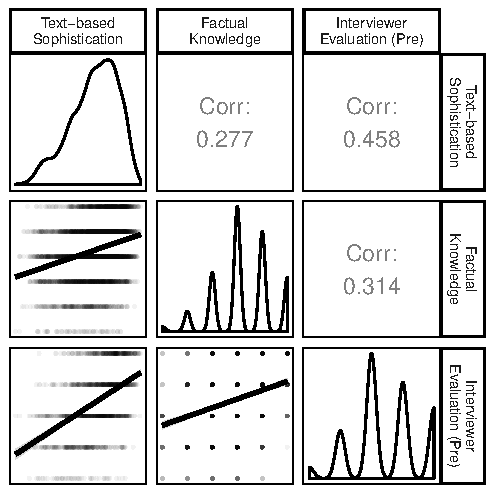
\includegraphics{../fig/corplot_pres.pdf}
\caption{Correlation matrix of conventional political knowledge metrics and the text-based sophistication measure. The plots on the diagonal display univariate densities for each variable. The panels in the lower triangular display the scatter plot of two measures as well as a linear fit. The upper triangular displays the correlation coefficient. All correlations reported are statistically significant with $p<.05$.}\label{fig:corplot}
\end{figure}

Interestingly, we observer a stronger correlation between text-based sophistication and interviewer evaluations than between factual knowledge and interviewer evaluations. The text-based measure therefore appears to capture characteristics that influence subjective assessments of sophistication. The interviewers certainly form their impressions throughout the entire survey, but it the complexity of a respondent's verbatim answers seems to be more influential than their performance on the factual knowledge questions.

Overall, while text-based sophistication and the alternative measures are clearly correlated, the relationship between each metric is far from perfect. To provide some intuition whether the variation in text-based sophistication is theoretically meaningful, I present an example of open-ended responses of two individuals who scored equally on the factual knowledge score (3 out of 5 correct responses), but varied highly in text-based sophistication. The results are presented in Table~\ref{tab:ex1}.

\begin{table}[ht]\footnotesize\centering
\begin{tabular}{l|p{6.5cm}|p{6.5cm}}
   \toprule
  & A: Low Sophistication Response & B: High Sophistication Response \\ 
   \midrule
   Obama (+) & The healthcare, keeping that and the financial aid, helping students. & I think he is honest, has good intentions. \\ \hdashline
     Obama (-) &  & I don't feel he is up for the job, he doesn't really know how to get things accomplished from idea to actual reality. \\ \hdashline
     Romney (+) &  & He comes across as an honest person and I feel that financially he would be better for the country. \\ \hdashline
     Romney (-) & By taking financial aid away from students, taking family type planning, healthcare type of help away. & I am a moderate conservative and there are some things about anti-gay rights that I don't support. \\ \hdashline
     Democrats (+) & Mostly the healthcare, mostly people do need healthcare and can't afford to pay insurance. Financial aid most people cant afford to go college. Main two things that I like is the help with education and to pay for insurance to go to doctor. & They do seem to be generally concerned with everyone, taking care of the country as a whole. \\ \hdashline
     Democrats (-) &  & They fight too much among themselves and I disagree with wealth redistribution. \\ \hdashline
     Republicans (+) &  & I agree with a lot of the conservative values and taking responsibility for one's own actions. \\ \hdashline
     Republicans (-) &  & They argue too much among themselves and don't accomplish very much. \\ 
    \bottomrule
 \end{tabular}
\caption{Example of open-ended responses for low and high scores on the text-based sophistication measure with equal factual knowledge scores (3 out of 5 correct responses). Column A displays the verbatim responses of an individual who scored low on the text-based sophistication measure and column B displays the verbatim responses of an individual who scored high on the text-based sophistication measure. Each row represents one of the likes/dislikes items included in the analysis. Note that the responses in this table were slightly redacted for readability (spelling errors removed, etc.).}\label{tab:ex1}
\end{table}

Each row in the table represents one of the open-ended responses (like/dislike for each candidate/party). Column A displays the responses of an individual who scored low on text-based sophistication and column B displays the responses of a high scoring individual. Cells are empty if a respondent refused to provide a response. Even though both individuals received are measured to be equal in their factual political knowledge, there are systematic differences in their response behavior that can be attributed to their political sophistication. Overall, respondent A provided a less elaborate response, only focused on two issues (health care and student loans), and did not report attitudes on multiple items. Compared to B, such a response pattern is suggestive of a less sophisticated political belief system. This result validation suggests that the variation in the sophistication measure captures meaningful differences in response behavior that clearly overlaps with traditional knowledge metrics while displaying some unique variation.

\section*{Validation: Political Sophistication Should Promote...}


\subsection*{... Engagement and Participation in Politics}

Political sophistication is commonly used as a determinant of engagement and participation in politics. Figure~\ref{fig:knoweff} presents the effects of each sophistication measure in the 2012 ANES on four dependent variables commonly related to political sophistication: internal efficacy, external efficacy, non-conventional participation, and turnout. The results for the first three dependent variables are based on linear regressions while the effects on turnout are estimated using a logit model. Each model equation includes a single sophistication measure while controlling for gender, education, income, age, race, religiosity, and survey mode (face-to-face vs. online). Each plot displays the difference in the expected value of the respective dependent variable for maximum and minimum values of each sophistication measure, while holding all other variables at their means.

\begin{figure}[h]\centering
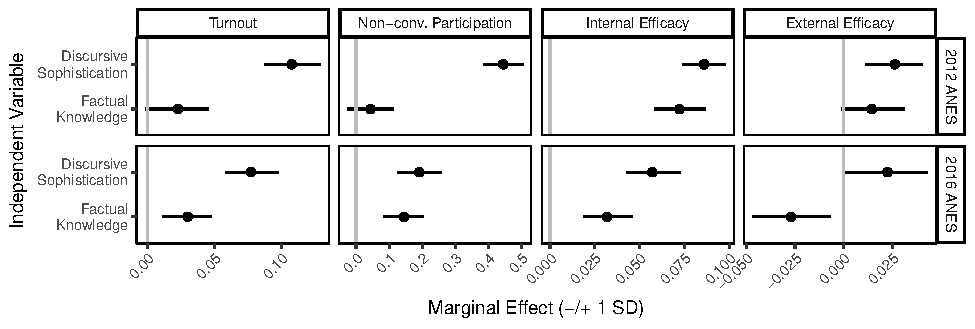
\includegraphics{../fig/knoweff_pres.pdf}
\caption{Effects of sophistication on internal efficacy, external efficacy, non-conventional participation, and turnout. For each dependent variable, the figure displays the difference in expected values between maximum and minimum levels of sophistication observed on each measure (including 95\% confidence intervals). Model estimates are based on OLS (internal efficacy, external efficacy, non-conventional participation) or logistic regressions (turnout). Each sophistication measure is included in a single equation while controlling for gender, education, income, age, race, church attendance, and survey mode. Full model results ar presented in the appendix, Tables \ref{tab:inteff} through \ref{tab:turnout}}\label{fig:knoweff}
\end{figure}
% TODO: add estimation controlling for all other factors

Overall, the sophistication metrics perform similarly as predictors of internal efficacy, external efficacy, non-conventional participation, and turnout. The effect of text-based sophistication on the participation measures is even stronger than the effect factual knowledge. This finding is especially noteworthy since the item batteries to measure factual political knowledge in the ANES are selected and validated based on their strong relationship with turnout and participation. 
% TODO: add citation for participation claim



\subsection*{... Precise Positioning of Parties and Candidates}

\begin{figure}[h]\centering
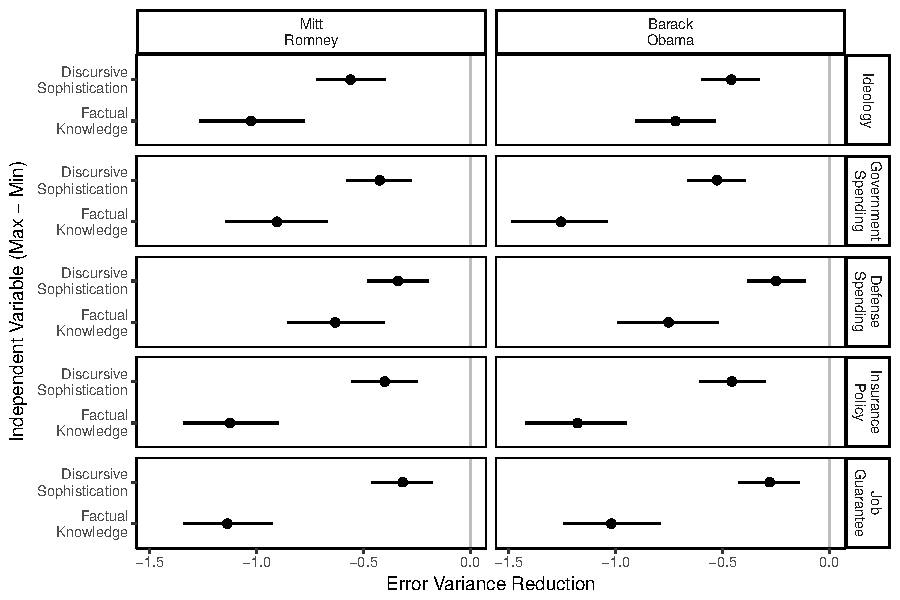
\includegraphics{../fig/hetreg.pdf}
\caption{Reduction in Error Variance}\label{fig:hetreg}
\end{figure}


\subsection*{... Stable Preferences}

\begin{figure}[h]\centering
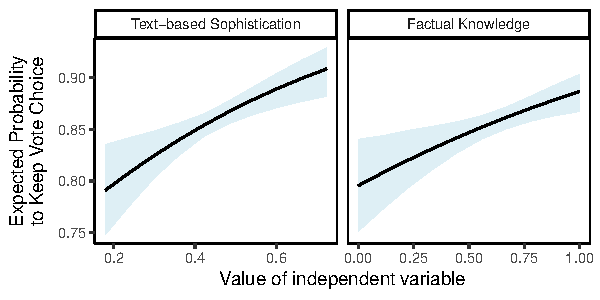
\includegraphics{../fig/prepost_exp.pdf}
\caption{Expected Probability to Keep Vote Choice}\label{fig:prepost}
\end{figure}

\subsection*{... Incorporation of New Information}
% TODO: How can I cite Jenn here? Add survey information (questionnaire etc.) in the appendix

The \textbf{factual knowledge} score in the YouGov data is based on a battery of eight items similar to the knowledge questions in the ANES. Additionally, the YouGov study included a task where respondents read a newspaper article about a fictional infectious disease and were subsequently asked to recall information provided in the article (e.g. regarding symptoms, modes of contraction etc.). I compute an additive index counting the pieces of information that were correctly recalled (\textbf{disease information}) as a measure of the ability to retrieve information from a news article on a non-partisan issue that is related to public health policies.


\begin{figure}[h]\centering
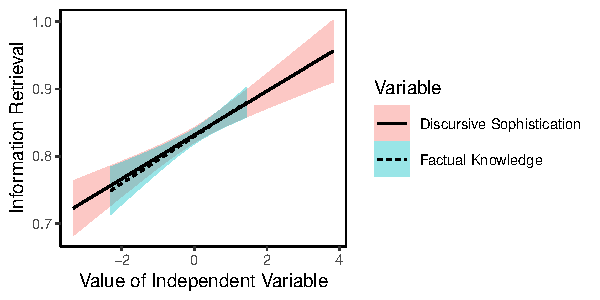
\includegraphics{../fig/yg_disease.pdf}
\caption{YouGov data -- Effect on disease retrieval.}\label{fig:yg_corplot}
\end{figure}


\subsection*{... Well Justified Political Decisions}


\begin{figure}[h]\centering
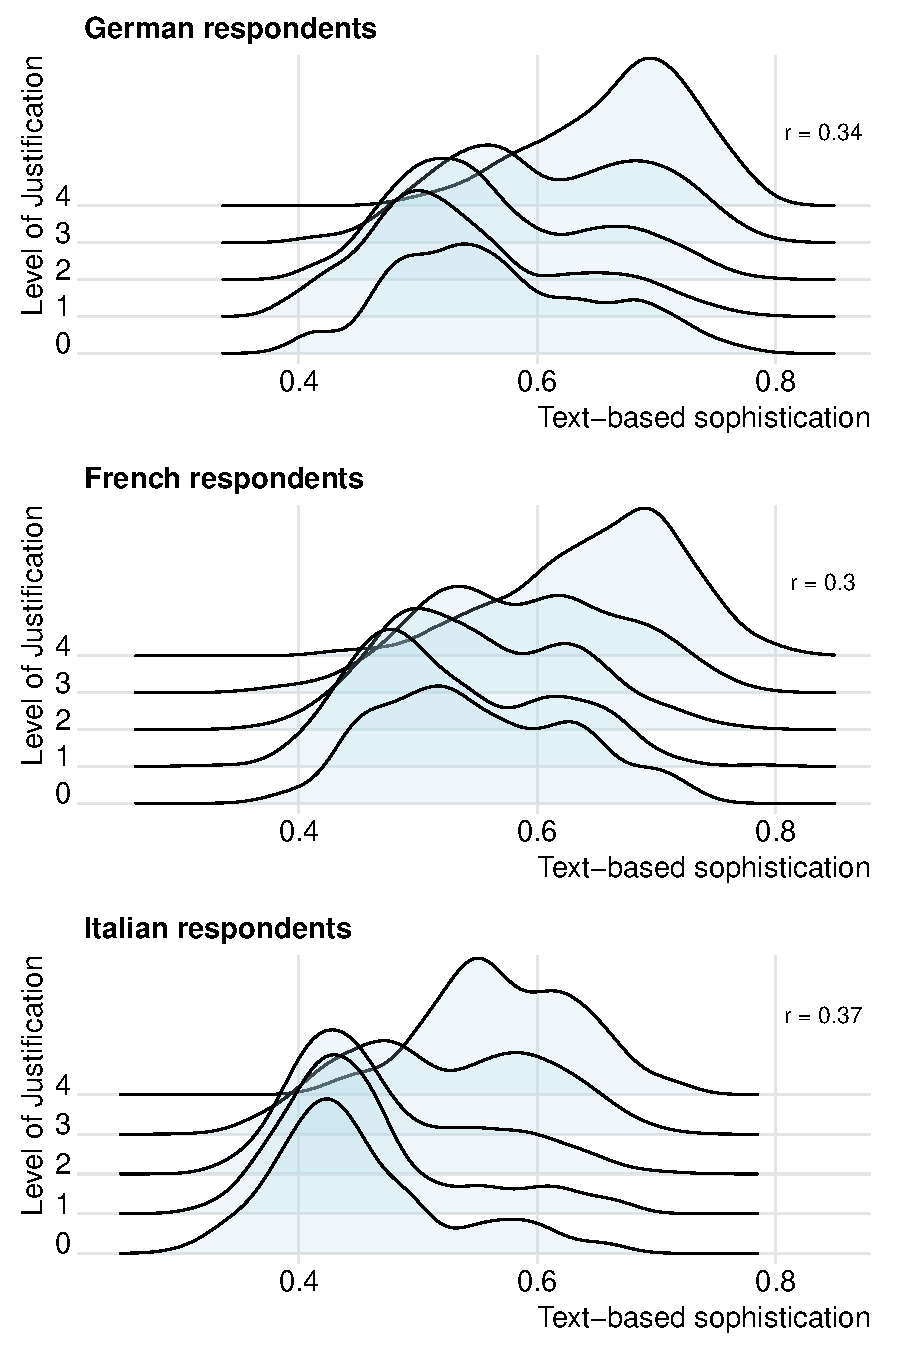
\includegraphics[scale=.6]{../fig/ggjoy.pdf}
\caption{Swiss data -- Political sophistication and level of justification.}\label{fig:swiss_ggjoy}
\end{figure}

%\section*{Robustness Checks: Personality and Open-Ended Responses}
% THIS IS FOR POST APSA! -> check whether text-based sophistication or polknow is more influenced by personality characteristics that should be unrelated with sophistication...


\section*{Application: The Gender Gap in Political Knowledge}
% APPENDIX: add additional analyses controlling for wordsum score, substantive results are unchanged

%One example for such potential misclassifications is the issue of gender differences in sophistication. On the basis of conventional factual knowledge scores, women frequently appear to be less informed about politics than men \citep{verba1997knowing,wolak2011roots}. However, some scholars suggested that these differences might be rooted in the conceptual and methodological issues related to the measurement approach. For example, \citet{mondak2004knowledge} argue that at least part of the gender gap in sophistication can be attributed to the fact that women are less likely to guess than men when facing a factual knowledge question for which they do not know an immediate answer. Others suggest that the gap can be attenuated by focusing on gender-relevant political knowledge \citep[e.g.,][]{dolan2011women} or by providing policy-specific information \citep[e.g.,][]{jerit2017revisiting}.


A common finding in research on political sophistication is the fact that women appear to be less knowledgeable about politics than men. For example, \citet{verba1997knowing} report that women score lower on political information, interest, and efficacy, which decreases their respective levels of political participation. Since gender differences in political information and interest can only partly be explained by resource-related factors such as individual levels of education, the authors diagnose a ``genuine difference in the taste for politics'' between men and women, which they suspect to be driven by socialization \citep[see also][]{wolak2011roots}.

Another explanation for the finding that disparities in resources (e.g., education) cannot fully account for gender differences is the fact that men and women benefit differently from the factors that increase political information \citep{dow2009gender}. As such, the gap is not only due to varying resource levels, but also due to differential gains from the resource itself. More broadly, this finding suggests that men and women consume political information through different channels \citep[see also][]{pietryka2013analysis}. Nevertheless, recent research showed that the gender gap can be substantially decreased given exposure to sufficient information \citep[e.g.][]{jerit2017revisiting} or through deliberation \citep{fraile2014does}.

Other scholars focused more closely on issues related to the measurement of political knowledge in order to explain the apparent gender gap. For example, \citet{mondak2004knowledge} suggest that women are more likely to report that they do not know the answer to a knowledge item if they are not completely certain, whereas men are more inclined to guess. Correcting for the systematic differences in the propensity to guess mitigates the gender gap in knowledge but does not eliminate it completely \citep[see also][]{lizotte2009explaining}. Based on their empirical evidence, \citet{mondak2004knowledge} elaborated on best practices regarding the measurement of political knowledge (e.g., using closed rather than open-ended knowledge items and discouraging `Don't Know' responses). Other related aspects of the survey context have also been shown to affect gender differences in political knowledge. For example, \citet{mcglone2006stereotype} present evidence that the gender gap is exacerbated in an environment that induces stereotype threat, for example if women are aware of the fact that the study focuses on gender differences or if they are interviewed by a male interviewer. However, gender differences are not only induced by \textit{how} researchers ask their questions, but also by the question \textit{content} itself. For example, \citet{dolan2011women} argues that the gap can be closed by focusing on gender-relevant political knowledge items such as information about women's representation in the federal government. Similarly, \citet{stolle2010women} report that the gender gap disappears when people are asked about more practical issues related to the government (e.g., benefits and services).

Overall, the gender gap has been shown to be influenced by how we ask for political information in surveys, as well as the kind of knowledge that is required for a correct response. Indeed, a comprehensive cross-national analysis of election studies in 47 countries between 1996 and 2011 suggests that question format and content account for large portions of the variance of gender disparities in political knowledge \citep{fortin2016cross}.


\subsection*{Study 1: 2012 American National Election Study}

How do men and women compare on the different metrics of political sophistication in the 2012 ANES? Figure~\ref{fig:meandiff} displays the average levels of text-based sophistication as well as the remaining metrics comparing both genders. While we observe a sizable gender gap for both conventional political knowledge measures, the difference is substantially smaller for text-based sophistication. Here, the gender gap is still statistically significant, but substantively inconsequential when compared to the remaining measures.

\begin{figure}[h]\centering
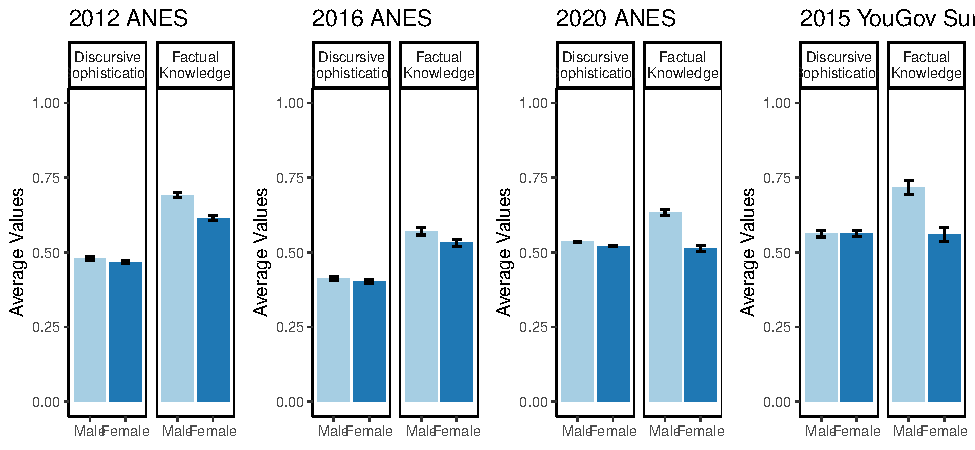
\includegraphics{../fig/meandiff_pres.pdf}
\caption{The gender gap in political sophistication. The figure displays mean levels of sophistication for each measure comparing men and women (including 95\% confidence intervals). The y-axis is scaled to range up to the maximum value observed in the data for each sophistication metric. All gender differences are statistically significant with $p<.05$.}\label{fig:meandiff}
\end{figure}

As described above, at least part of the gender gap can be attributed to real differences in resources relevant to political information (e.g., education). Accordingly, we need to control for common determinants of political knowledge across all available measures to provide a more comprehensive examination of potential gender differences. Previous studies consistently showed that political knowledge is positively related to high media exposure, frequent political discussions, education, and income. Furthermore, I include age, race, religiosity, and survey mode (face-to-face vs. online) as additional control variables. Figure~\ref{fig:determinants} displays the coefficients of regression models with each knowledge/sophistication measure as the dependent variable.

\begin{figure}[h]\centering
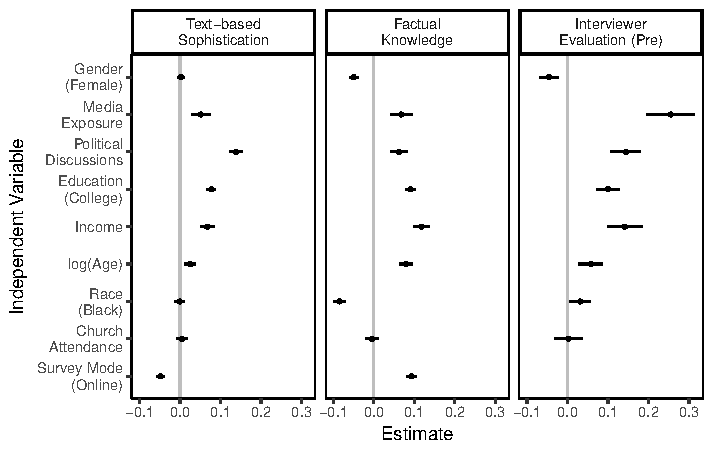
\includegraphics{../fig/determinants_pres.pdf}
\caption{Common determinants of political sophistication. Estimates are OLS regression coefficients with 95\% confidence intervals. Dependent variables are the text-based sophistication measure as well as conventional metrics of political knowledge. Full model results are presented in the appendix, Table~\ref{tab:determinants}}\label{fig:determinants}
\end{figure}
% NOTE: rescale knowledge variables to unit variance? the effects would be better to compare...

After controlling for common determinants, text-based sophistication reveals no significant differences between men and women. On the other hand, we still observe the gender gap using all remaining political knowledge metrics considered here. As such, women might not score as highly on political quizzes (partly because they are less likely to guess rather express lack of knowledge), but they do not differ substantially in complexity and sophistication when they describe their political preferences.

The patterns for the remaining determinants are quite similar across different dependent variables. Knowledge and sophistication is significantly higher among respondents who are more exposed to political news media, discuss politics frequently, are more educated, and have higher income. An interesting deviation, however, is the effect of survey mode. For factual knowledge questions, we observe that respondents in online surveys score significantly higher than individuals in face-to-face interviews. This difference could be explained by the fact that individuals are able to look up responses to factual knowledge questions while taking an online survey \citep[see also][]{clifford2016cheating}. For the text-based measure, on the other hand, we see that individuals appear to score lower on sophistication in online surveys. Respondents in online surveys therefore seem less willing to elaborate on their attitudes. Overall, the fact that the determinants of political sophistication are very consistent across models lends additional validity to the text-based measure.





% REVISE: Make a reference to Jenn's study, which found that gender differences disappear if information is provided to respondents

% TODO: add section with LI survey data?
% issue: doesn't contain conventional political knowledge score
% but I could examine party identification as a determinant of political sophistication

% IDEA: out-party sophistication vs. in-party sophistication?
% I could split up the measure by in-party vs. out-party and examine
% the difference as an indicator of political tolerance etc.
% maybe there is an item that examines whether people would revise their vote choice etc. after the election and I could compare traditional knowledge vs. text-based sophistication.


\section*{Conclusion}
% lot's of potential extensions, think about standardizing the measure to make it more comparable across contexts
% Zaller argues that it captures what actually got into people's minds... that's a perfect argument for open-ended responses! check also the druckman paper.
% Make a connection to political competence, we shouldn't care as much about political knowledge that is favored by elites, but rather examine whether individuals are able to discuss their political views in a coherent way. Seen that way, one could make an argument that political competence captures the extent to which individuals are able to incorporate new information.
% What is a competent citizen? One who has good reasons for his or her attitudes... we can measure that when examining how repondents talk about their political beliefs.

Political scientists should worry less about pure levels of \textit{information}, but rather focus on the necessary conditions for individuals to make \textit{competent} decisions. Competence in the context of political decision-making and voting requires citizens to hold informed attitudes about their representatives. Factual knowledge about political institutions might be a useful proxy for competence in certain scenarios. However, it cannot address directly whether individuals are sufficiently opinionated about political actors they try to hold accountable. In comparison, the text-based sophistication measure proposed here is agnostic about the specific contents of individual beliefs, but directly captures the structure and complexity in attitude expression.

The findings presented in this paper show that conventional knowledge indices and the text-based measure share a substantial amount of variance. However, they are far from being identical and capture different aspects of sophistication. Most importantly, using the text-based measure, any evidence for the gender gap commonly reported using factual knowledge scales disappears. Women might know fewer facts about political institutions, but they do not differ substantively in the complexity of their expressed political beliefs.


\singlespacing
\bibliographystyle{/data/Dropbox/Uni/Lit/apsr2006}
\bibliography{/data/Dropbox/Uni/Lit/Literature}

\clearpage
\section*{Appendix A: Open-ended Responses in ANES}
\renewcommand\thefigure{A.\arabic{figure}}
\renewcommand\thetable{A.\arabic{table}}
\setcounter{figure}{0}
\setcounter{table}{0}


% COMBINE: combine histograms etc. for different datasets in a single plot...

\begin{figure}[h]\centering
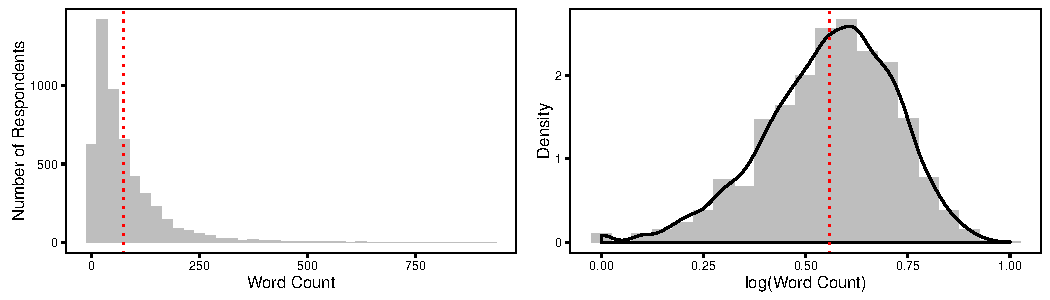
\includegraphics{../fig/wc.pdf}
\caption{Histogram of total word count in the collection of open-ended responses for each individual (left panel) and distribution of logged word count used in the text-based sophistication measure (right panel, re-scaled to range from 0 to 1). Dashed red lines indicate mean values. Most respondents provide brief statements when they describe their attitudes towards political parties and candidates. The mean response length to all 8 questions is about 75 words, so an average response to a single question consisted of less than 10 words, omitting respondents who did not provide any information.}\label{fig:wc}
\end{figure}

\begin{figure}[h]\centering
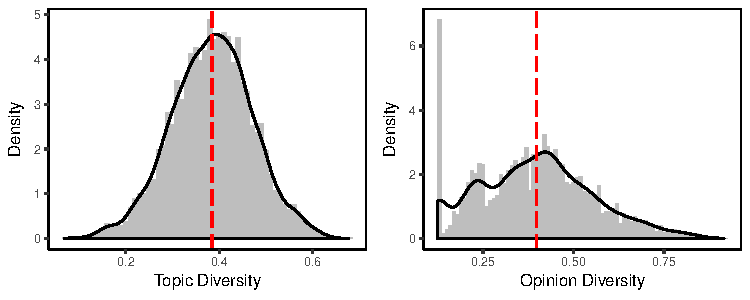
\includegraphics{../fig/diversity.pdf}
\caption{Histogram and density of the topic diversity (left panel) and opinion diversity (right panel) measure. Dashed red lines indicate mean values. The spike at 0 for opinion diversity are due to the fact that a large proportion of respondents only answered a single open-ended question.}\label{fig:diversity}
\end{figure}


\clearpage
\section*{Appendix B: Open-ended Responses in YouGov Data}
\renewcommand\thefigure{B.\arabic{figure}}
\renewcommand\thetable{B.\arabic{table}}
\setcounter{figure}{0}
\setcounter{table}{0}

\begin{figure}[h]\centering
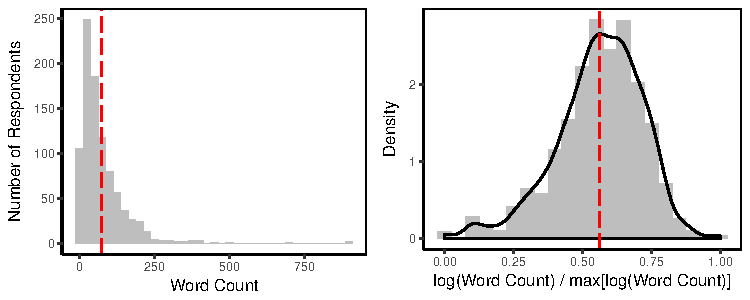
\includegraphics{../fig/yg_wc.pdf}
\caption{Histogram of total word count in the collection of open-ended responses for each individual (left panel) and distribution of logged word count used in the text-based sophistication measure (right panel, re-scaled to range from 0 to 1). Dashed red lines indicate mean values. Most respondents provide brief statements when they describe their attitudes towards political parties and candidates. The mean response length to all 8 questions is about 73 words, so an average response to a single question consisted of approximately 18 words, omitting respondents who did not provide any information.}\label{fig:yg_wc}
\end{figure}

\begin{figure}[h]\centering
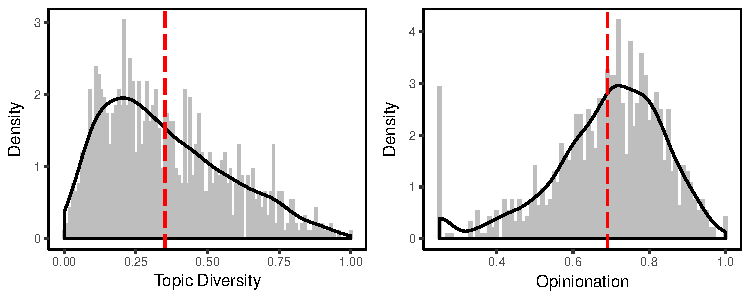
\includegraphics{../fig/yg_diversity.pdf}
\caption{Histogram and density of the topic diversity (left panel) and opinion diversity (right panel) measure. Dashed red lines indicate mean values. The spike at 0 for opinion diversity are due to the fact that a large proportion of respondents only answered a single open-ended question.}\label{fig:yg_diversity}
\end{figure}


%\clearpage
%\section*{Appendix C: YouGov Correlation Matrix}
%
%Figure~\ref{fig:yg_corplot} examines the distribution of each measure of political knowledge as well as their respective correlations in the YouGov data. Again, we observe that text-based sophistication and factual political knowledge are positively correlated, which indicates that the text-based sophistication measure overlaps with traditional knowledge metrics while capturing unique variation in individual response behavior. Interestingly, there appears to be a stronger relationship between text-based sophistication and disease information than between factual political knowledge and disease information.
%
%\begin{figure}[h]\centering
%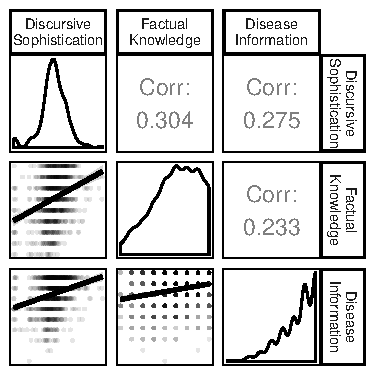
\includegraphics{../fig/yg_corplot.pdf}
%\caption{YouGov data -- Correlation matrix of text-based sophistication, a conventional political knowledge metric, and disease information retrieval. The plots on the diagonal display univariate densities for each variable. The panels in the lower triangular display the scatter plot of two measures as well as a linear fit. The upper triangular displays the correlation coefficient. All correlations reported are statistically significant with $p<.05$.}\label{fig:yg_corplot}
%\end{figure}
%
%Recall that the disease information score can be interpreted as an indicator of the ability to retrieve specific information provided in a news article about a public health issue. It could be argued that text-based sophistication is more similar to the disease information score in that it captures the extent to which participants were able to recall political information that is relevant to their own attitudes. Conventional knowledge scores, on the other hand, inquire about specific that are not necessarily relevant to derive well-informed attitudes about political issues.



%\subsection*{Appendix D: Gender Gap Replication -- 2015 YouGov Data}
%
%Next, I examine whether the results regarding the gender gap observed in Study 1 are replicated in the YouGov data. Figure~\ref{fig:yg_meandiff} compares the alternative measures of political knowledge and sophistication for men and women. As before, we observe a significant gender gap in factual knowledge (middle panel), which disappears using the text-based measure (left panel). Furthermore, there is no apparent gender gap in disease information retrieval. If anything, women are able to recall slightly more accurate information about the infectious disease described in the news article. This result is consistent with recent research by \citet{jerit2017revisiting}, which suggests that knowledge gaps between men and women disappear upon receiving sufficient information.
%
%\begin{figure}[h]\centering
%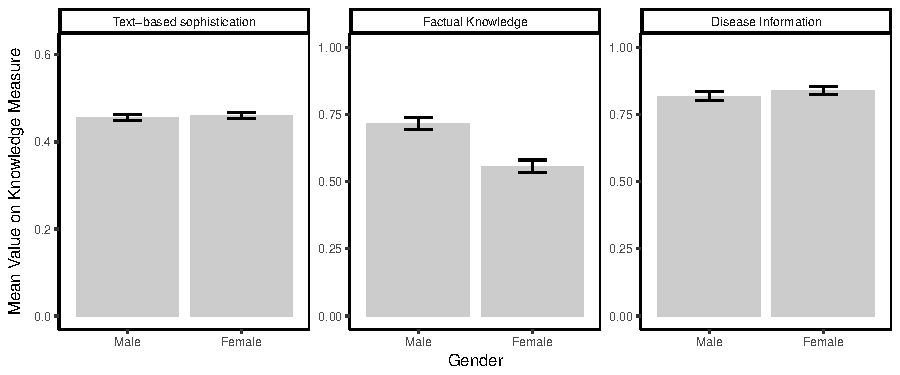
\includegraphics{../fig/yg_meandiff.pdf}
%\caption{YouGov data -- The gender gap in political sophistication. The figure displays mean levels of sophistication for each measure comparing men and women (including 95\% confidence intervals). The y-axis is scaled to range up to the maximum value observed in the data for each sophistication metric. The gender difference in factual knowledge is statistically significant with $p<.05$.}\label{fig:yg_meandiff}
%\end{figure}
%
%A skeptical reader may again argue that the difference in factual knowledge between men and women could potentially be explained by systematic differences in resource-related factors. As such, we need to examine whether the gender gap persists even after controlling for covariates that might influence political knowledge. Similar to the analyses discussed in Study 1, Figure~\ref{fig:yg_determinants} presents the results of linear regressions predicting each measure as a function of gender, education, income, age, race, and religiosity.
%
%\begin{figure}[h]\centering
%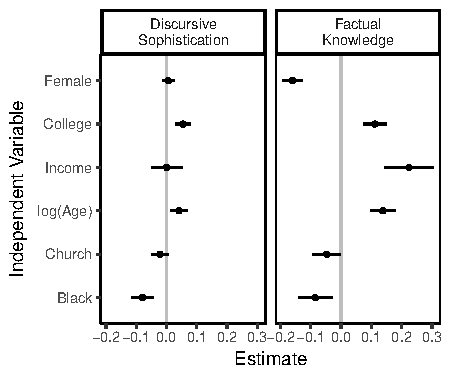
\includegraphics{../fig/yg_determinants.pdf}
%\caption{Common determinants of political sophistication -- Replication using YouGov data. Estimates are OLS regression coefficients with 95\% confidence intervals. Dependent variables are the text-based sophistication measure, factual political knowledge as well as knowledge about a fictional disease that was presented as part of the study. Full model results are presented in the appendix, Table~\ref{tab:yg_determinants}}\label{fig:yg_determinants}
%\end{figure}
%
%As before, men do not perform better than women on text-based sophistication or disease information retrieval in a multivariate setting. However, the gender gap in factual political knowledge persists and is substantively as well as statistically significant. The remaining determinants of sophistication/knowledge are similar across measures (except for family income). Interestingly, the observed pattern of effects on text-based sophistication is strikingly similar to the effects on information retrieval about the fictional disease. This result reinforces the conclusion that text-based sophistication and disease information retrieval in the YouGov study share common characteristics in the sense that they capture how individuals recall considerations that are relevant to their own attitudes rather than inquiring about facts related to political institutions and elites that are extraneous to the issues at hand.




%\clearpage
%\section*{Appendix E: Tables of Model Estimates}
%\renewcommand\thefigure{C.\arabic{figure}}
%\renewcommand\thetable{C.\arabic{table}}
%\setcounter{figure}{0}
%\setcounter{table}{0}
%
%
% Table created by stargazer v.5.2 by Marek Hlavac, Harvard University. E-mail: hlavac at fas.harvard.edu
% Date and time: Fri, Mar 31, 2017 - 11:40:40 PM
% Requires LaTeX packages: dcolumn 
\begin{table}[ht] \centering 
  \caption{Effects on Internal Efficacy} 
  \label{tab:inteff} 
\scriptsize 
\begin{tabular}{@{\extracolsep{-5pt}}lD{.}{.}{-3} D{.}{.}{-3} D{.}{.}{-3} D{.}{.}{-3} D{.}{.}{-3} D{.}{.}{-3} } 
\\[-1.8ex]\hline 
\hline \\[-1.8ex] 
 & \multicolumn{6}{c}{\textit{Dependent variable:}} \\ 
\cline{2-7} 
\\[-1.8ex] & \multicolumn{6}{c}{Iternal Efficacy} \\ 
\\[-1.8ex] & \multicolumn{1}{c}{(1)} & \multicolumn{1}{c}{(2)} & \multicolumn{1}{c}{(3)} & \multicolumn{1}{c}{(4)} & \multicolumn{1}{c}{(5)} & \multicolumn{1}{c}{(6)}\\ 
\hline \\[-1.8ex] 
 Text-based & 0.554^{***} &  &  &  &  &  \\ 
  & (0.035) &  &  &  &  &  \\ 
  Factual &  & 0.237^{***} &  &  &  &  \\ 
  &  & (0.015) &  &  &  &  \\ 
  Office &  &  & 0.248^{***} &  &  &  \\ 
  &  &  & (0.011) &  &  &  \\ 
  Majorities &  &  &  & 0.140^{***} &  &  \\ 
  &  &  &  & (0.008) &  &  \\ 
  Eval. (Pre) &  &  &  &  & 0.361^{***} &  \\ 
  &  &  &  &  & (0.019) &  \\ 
  Eval. (Post) &  &  &  &  &  & 0.285^{***} \\ 
  &  &  &  &  &  & (0.020) \\ 
  Sex (Female) & -0.062^{***} & -0.050^{***} & -0.052^{***} & -0.053^{***} & -0.038^{***} & -0.040^{***} \\ 
  & (0.006) & (0.006) & (0.006) & (0.006) & (0.010) & (0.010) \\ 
  Education (College) & 0.056^{***} & 0.055^{***} & 0.038^{***} & 0.063^{***} & 0.035^{**} & 0.044^{***} \\ 
  & (0.006) & (0.006) & (0.007) & (0.006) & (0.011) & (0.012) \\ 
  log(Age) & 0.019^{*} & 0.008 & 0.009 & 0.010 & -0.016 & -0.005 \\ 
  & (0.008) & (0.008) & (0.008) & (0.008) & (0.012) & (0.013) \\ 
  Race (Black) & 0.041^{***} & 0.058^{***} & 0.048^{***} & 0.042^{***} & 0.050^{***} & 0.059^{***} \\ 
  & (0.008) & (0.008) & (0.008) & (0.008) & (0.011) & (0.011) \\ 
  Church Attendance & 0.005 & 0.008 & 0.013 & 0.005 & -0.003 & -0.009 \\ 
  & (0.008) & (0.008) & (0.008) & (0.009) & (0.014) & (0.015) \\ 
  Survey Mode (Online) & 0.047^{***} & 0.009 & -0.009 & 0.001 &  &  \\ 
  & (0.006) & (0.006) & (0.007) & (0.007) &  &  \\ 
  Constant & 0.179^{***} & 0.368^{***} & 0.442^{***} & 0.444^{***} & 0.377^{***} & 0.400^{***} \\ 
  & (0.033) & (0.030) & (0.030) & (0.031) & (0.044) & (0.047) \\ 
 \hline \\[-1.8ex] 
Observations & \multicolumn{1}{c}{5,135} & \multicolumn{1}{c}{5,135} & \multicolumn{1}{c}{4,816} & \multicolumn{1}{c}{4,816} & \multicolumn{1}{c}{1,743} & \multicolumn{1}{c}{1,647} \\ 
R$^{2}$ & \multicolumn{1}{c}{0.114} & \multicolumn{1}{c}{0.116} & \multicolumn{1}{c}{0.160} & \multicolumn{1}{c}{0.128} & \multicolumn{1}{c}{0.228} & \multicolumn{1}{c}{0.170} \\ 
\hline 
\hline \\[-1.8ex] 
\textit{Note:}  & \multicolumn{6}{r}{$^{*}$p$<$0.05; $^{**}$p$<$0.01; $^{***}$p$<$0.001} \\ 
\end{tabular} 
\end{table} 

%
% Table created by stargazer v.5.2 by Marek Hlavac, Harvard University. E-mail: hlavac at fas.harvard.edu
% Date and time: Thu, Jun 22, 2017 - 04:21:44 PM
% Requires LaTeX packages: dcolumn 
\begin{table}[ht] \centering 
  \caption{Effects of sophistication -- OLS models predicting external efficacy 
          based on different sophistication 
          measures. Positive coefficients indicate higher self-reported external efficacy. 
          Standard errors in parentheses. Estimates are used for Figure~\ref{fig:knoweff} 
          in the main text.} 
  \label{tab:exteff} 
\scriptsize 
\begin{tabular}{@{\extracolsep{-5pt}}lD{.}{.}{-3} D{.}{.}{-3} D{.}{.}{-3} D{.}{.}{-3} D{.}{.}{-3} D{.}{.}{-3} } 
\\[-1.8ex]\hline 
\hline \\[-1.8ex] 
 & \multicolumn{6}{c}{\textit{Dependent variable:}} \\ 
\cline{2-7} 
\\[-1.8ex] & \multicolumn{6}{c}{External Efficacy} \\ 
\hline \\[-1.8ex] 
 Text-based & 0.110^{**} &  &  &  &  &  \\ 
  & (0.041) &  &  &  &  &  \\ 
  Factual &  & 0.049^{**} &  &  &  &  \\ 
  &  & (0.017) &  &  &  &  \\ 
  Office &  &  & 0.084^{***} &  &  &  \\ 
  &  &  & (0.013) &  &  &  \\ 
  Majorities &  &  &  & 0.044^{***} &  &  \\ 
  &  &  &  & (0.010) &  &  \\ 
  Eval. (Pre) &  &  &  &  & 0.136^{***} &  \\ 
  &  &  &  &  & (0.026) &  \\ 
  Eval. (Post) &  &  &  &  &  & 0.149^{***} \\ 
  &  &  &  &  &  & (0.027) \\ 
  Sex (Female) & 0.014^{*} & 0.016^{*} & 0.015^{*} & 0.015^{*} & 0.023 & 0.023 \\ 
  & (0.007) & (0.007) & (0.007) & (0.007) & (0.013) & (0.014) \\ 
  Education (College) & 0.041^{***} & 0.041^{***} & 0.033^{***} & 0.040^{***} & 0.064^{***} & 0.057^{***} \\ 
  & (0.008) & (0.008) & (0.008) & (0.008) & (0.016) & (0.016) \\ 
  Income & 0.023 & 0.021 & 0.012 & 0.021 & 0.006 & 0.002 \\ 
  & (0.012) & (0.012) & (0.013) & (0.013) & (0.025) & (0.025) \\ 
  log(Age) & -0.008 & -0.011 & -0.013 & -0.012 & -0.051^{**} & -0.048^{**} \\ 
  & (0.009) & (0.009) & (0.010) & (0.010) & (0.016) & (0.017) \\ 
  Race (Black) & 0.077^{***} & 0.080^{***} & 0.078^{***} & 0.076^{***} & 0.058^{***} & 0.058^{***} \\ 
  & (0.009) & (0.009) & (0.009) & (0.009) & (0.015) & (0.015) \\ 
  Church Attendance & 0.048^{***} & 0.049^{***} & 0.053^{***} & 0.050^{***} & 0.045^{*} & 0.042^{*} \\ 
  & (0.010) & (0.010) & (0.010) & (0.010) & (0.019) & (0.020) \\ 
  Survey Mode (Online) & -0.036^{***} & -0.043^{***} & -0.055^{***} & -0.051^{***} &  &  \\ 
  & (0.008) & (0.008) & (0.008) & (0.008) &  &  \\ 
  Constant & 0.369^{***} & 0.407^{***} & 0.434^{***} & 0.432^{***} & 0.462^{***} & 0.455^{***} \\ 
  & (0.038) & (0.035) & (0.036) & (0.037) & (0.061) & (0.063) \\ 
 \hline \\[-1.8ex] 
Observations & \multicolumn{1}{c}{4,993} & \multicolumn{1}{c}{4,993} & \multicolumn{1}{c}{4,694} & \multicolumn{1}{c}{4,694} & \multicolumn{1}{c}{1,653} & \multicolumn{1}{c}{1,569} \\ 
R$^{2}$ & \multicolumn{1}{c}{0.040} & \multicolumn{1}{c}{0.040} & \multicolumn{1}{c}{0.048} & \multicolumn{1}{c}{0.044} & \multicolumn{1}{c}{0.053} & \multicolumn{1}{c}{0.053} \\ 
\hline 
\hline \\[-1.8ex] 
\textit{Note:}  & \multicolumn{6}{r}{$^{*}$p$<$0.05; $^{**}$p$<$0.01; $^{***}$p$<$0.001} \\ 
\end{tabular} 
\end{table} 

%
% Table created by stargazer v.5.2 by Marek Hlavac, Harvard University. E-mail: hlavac at fas.harvard.edu
% Date and time: Mon, Apr 03, 2017 - 04:16:07 PM
% Requires LaTeX packages: dcolumn 
\begin{table}[ht] \centering 
  \caption{Effects of sophistication -- OLS models predicting non-conventional 
          particpation (protest, signing 
          petitions, etc.) based on different sophistication 
          measures. Positive coefficients indicate higher levels of participation. 
          Standard errors in parentheses. Estimates are used for Figure~\ref{fig:knoweff} 
          in the main text.} 
  \label{tab:nonconv} 
\scriptsize 
\begin{tabular}{@{\extracolsep{-5pt}}lD{.}{.}{-3} D{.}{.}{-3} D{.}{.}{-3} D{.}{.}{-3} D{.}{.}{-3} D{.}{.}{-3} } 
\\[-1.8ex]\hline 
\hline \\[-1.8ex] 
 & \multicolumn{6}{c}{\textit{Dependent variable:}} \\ 
\cline{2-7} 
\\[-1.8ex] & \multicolumn{6}{c}{Non-conventional Participation} \\ 
\hline \\[-1.8ex] 
 Text-based & 1.150^{***} &  &  &  &  &  \\ 
  & (0.084) &  &  &  &  &  \\ 
  Factual &  & 0.212^{***} &  &  &  &  \\ 
  &  & (0.036) &  &  &  &  \\ 
  Office &  &  & 0.331^{***} &  &  &  \\ 
  &  &  & (0.027) &  &  &  \\ 
  Majorities &  &  &  & 0.159^{***} &  &  \\ 
  &  &  &  & (0.019) &  &  \\ 
  Eval. (Pre) &  &  &  &  & 0.452^{***} &  \\ 
  &  &  &  &  & (0.048) &  \\ 
  Eval. (Post) &  &  &  &  &  & 0.445^{***} \\ 
  &  &  &  &  &  & (0.048) \\ 
  Sex (Female) & 0.007 & 0.014 & 0.022 & 0.017 & 0.025 & 0.027 \\ 
  & (0.014) & (0.014) & (0.014) & (0.014) & (0.024) & (0.024) \\ 
  Education (College) & 0.089^{***} & 0.122^{***} & 0.088^{***} & 0.125^{***} & 0.103^{***} & 0.099^{***} \\ 
  & (0.016) & (0.016) & (0.016) & (0.015) & (0.028) & (0.028) \\ 
  log(Age) & 0.035 & 0.040^{*} & 0.027 & 0.033 & -0.052 & -0.047 \\ 
  & (0.019) & (0.020) & (0.019) & (0.019) & (0.030) & (0.030) \\ 
  Race (Black) & 0.036 & 0.044^{*} & 0.040^{*} & 0.030 & -0.020 & -0.011 \\ 
  & (0.018) & (0.019) & (0.019) & (0.019) & (0.027) & (0.027) \\ 
  Church Attendance & 0.028 & 0.035 & 0.041^{*} & 0.031 & 0.047 & 0.041 \\ 
  & (0.020) & (0.020) & (0.020) & (0.020) & (0.035) & (0.035) \\ 
  Survey Mode (Online) & 0.103^{***} & 0.051^{**} & 0.019 & 0.039^{*} &  &  \\ 
  & (0.015) & (0.016) & (0.016) & (0.016) &  &  \\ 
  Constant & -0.392^{***} & 0.032 & 0.130 & 0.121 & 0.275^{*} & 0.287^{*} \\ 
  & (0.080) & (0.074) & (0.073) & (0.074) & (0.112) & (0.112) \\ 
 \hline \\[-1.8ex] 
Observations & \multicolumn{1}{c}{4,809} & \multicolumn{1}{c}{4,809} & \multicolumn{1}{c}{4,809} & \multicolumn{1}{c}{4,809} & \multicolumn{1}{c}{1,638} & \multicolumn{1}{c}{1,638} \\ 
R$^{2}$ & \multicolumn{1}{c}{0.068} & \multicolumn{1}{c}{0.038} & \multicolumn{1}{c}{0.061} & \multicolumn{1}{c}{0.045} & \multicolumn{1}{c}{0.078} & \multicolumn{1}{c}{0.075} \\ 
\hline 
\hline \\[-1.8ex] 
\textit{Note:}  & \multicolumn{6}{r}{$^{*}$p$<$0.05; $^{**}$p$<$0.01; $^{***}$p$<$0.001} \\ 
\end{tabular} 
\end{table} 

%
% Table created by stargazer v.5.2 by Marek Hlavac, Harvard University. E-mail: hlavac at fas.harvard.edu
% Date and time: Fri, Mar 31, 2017 - 11:40:45 PM
% Requires LaTeX packages: dcolumn 
\begin{table}[ht] \centering 
  \caption{Effects on Turnout (Logit)} 
  \label{tab:turnout} 
\scriptsize 
\begin{tabular}{@{\extracolsep{-5pt}}lD{.}{.}{-3} D{.}{.}{-3} D{.}{.}{-3} D{.}{.}{-3} D{.}{.}{-3} D{.}{.}{-3} } 
\\[-1.8ex]\hline 
\hline \\[-1.8ex] 
 & \multicolumn{6}{c}{\textit{Dependent variable:}} \\ 
\cline{2-7} 
\\[-1.8ex] & \multicolumn{6}{c}{Turnout} \\ 
\hline \\[-1.8ex] 
 Text-based & 5.521^{***} &  &  &  &  &  \\ 
  & (0.487) &  &  &  &  &  \\ 
  Factual &  & 1.376^{***} &  &  &  &  \\ 
  &  & (0.197) &  &  &  &  \\ 
  Office &  &  & 2.213^{***} &  &  &  \\ 
  &  &  & (0.180) &  &  &  \\ 
  Majorities &  &  &  & 1.152^{***} &  &  \\ 
  &  &  &  & (0.108) &  &  \\ 
  Eval. (Pre) &  &  &  &  & 2.942^{***} &  \\ 
  &  &  &  &  & (0.271) &  \\ 
  Eval. (Post) &  &  &  &  &  & 2.831^{***} \\ 
  &  &  &  &  &  & (0.276) \\ 
  Sex (Female) & 0.045 & 0.054 & 0.120 & 0.112 & 0.143 & 0.145 \\ 
  & (0.082) & (0.081) & (0.083) & (0.082) & (0.130) & (0.130) \\ 
  Education (College) & 0.699^{***} & 0.804^{***} & 0.615^{***} & 0.815^{***} & 0.723^{***} & 0.679^{***} \\ 
  & (0.104) & (0.103) & (0.105) & (0.102) & (0.177) & (0.176) \\ 
  log(Age) & 1.086^{***} & 1.061^{***} & 0.993^{***} & 1.011^{***} & 0.773^{***} & 0.759^{***} \\ 
  & (0.102) & (0.102) & (0.103) & (0.103) & (0.156) & (0.156) \\ 
  Race (Black) & 0.649^{***} & 0.728^{***} & 0.682^{***} & 0.629^{***} & 0.772^{***} & 0.808^{***} \\ 
  & (0.115) & (0.116) & (0.114) & (0.114) & (0.157) & (0.156) \\ 
  Church Attendance & 0.717^{***} & 0.738^{***} & 0.767^{***} & 0.721^{***} & 0.830^{***} & 0.753^{***} \\ 
  & (0.125) & (0.124) & (0.125) & (0.125) & (0.199) & (0.198) \\ 
  Survey Mode (Online) & 0.719^{***} & 0.412^{***} & 0.234^{**} & 0.281^{**} &  &  \\ 
  & (0.086) & (0.086) & (0.087) & (0.088) &  &  \\ 
  Constant & -6.628^{***} & -4.563^{***} & -4.002^{***} & -3.947^{***} & -4.101^{***} & -3.800^{***} \\ 
  & (0.440) & (0.384) & (0.388) & (0.387) & (0.587) & (0.579) \\ 
 \hline \\[-1.8ex] 
Observations & \multicolumn{1}{c}{4,831} & \multicolumn{1}{c}{4,831} & \multicolumn{1}{c}{4,812} & \multicolumn{1}{c}{4,812} & \multicolumn{1}{c}{1,647} & \multicolumn{1}{c}{1,645} \\ 
Akaike Inf. Crit. & \multicolumn{1}{c}{3,937.628} & \multicolumn{1}{c}{4,022.502} & \multicolumn{1}{c}{3,893.755} & \multicolumn{1}{c}{3,948.129} & \multicolumn{1}{c}{1,550.512} & \multicolumn{1}{c}{1,563.228} \\ 
\hline 
\hline \\[-1.8ex] 
\textit{Note:}  & \multicolumn{6}{r}{$^{*}$p$<$0.05; $^{**}$p$<$0.01; $^{***}$p$<$0.001} \\ 
\end{tabular} 
\end{table} 

%
% Table created by stargazer v.5.2 by Marek Hlavac, Harvard University. E-mail: hlavac at fas.harvard.edu
% Date and time: Wed, Jun 14, 2017 - 11:02:19 AM
% Requires LaTeX packages: dcolumn 
\begin{table}[ht] \centering 
  \caption{Determinants of political knowledge -- OLS models predicting different 
          political sophistication measures.
          Positive coefficients indicate higher sophistication. 
          Standard errors in parentheses. Estimates are used for Figure~\ref{fig:determinants} 
          in the main text.} 
  \label{tab:determinants} 
\scriptsize 
\begin{tabular}{@{\extracolsep{-5pt}}lD{.}{.}{-3} D{.}{.}{-3} D{.}{.}{-3} D{.}{.}{-3} D{.}{.}{-3} D{.}{.}{-3} } 
\\[-1.8ex]\hline 
\hline \\[-1.8ex] 
 & \multicolumn{6}{c}{Dependent Variable: Political Knowledge Measure} \\ 
\cline{2-7} 
\\[-1.8ex] & \multicolumn{1}{c}{Text-based} & \multicolumn{1}{c}{Factual} & \multicolumn{1}{c}{Office} & \multicolumn{1}{c}{Majorities} & \multicolumn{1}{c}{Eval. (Pre)} & \multicolumn{1}{c}{Eval. (Post)} \\ 
\hline \\[-1.8ex] 
 Gender (Female) & -0.002 & -0.049^{***} & -0.045^{***} & -0.082^{***} & -0.046^{***} & -0.052^{***} \\ 
  & (0.002) & (0.006) & (0.007) & (0.011) & (0.012) & (0.012) \\ 
  Media Exposure & 0.024^{***} & 0.069^{***} & 0.159^{***} & 0.193^{***} & 0.255^{***} & 0.192^{***} \\ 
  & (0.006) & (0.014) & (0.018) & (0.026) & (0.030) & (0.030) \\ 
  Political Discussions & 0.056^{***} & 0.062^{***} & 0.195^{***} & 0.200^{***} & 0.144^{***} & 0.174^{***} \\ 
  & (0.004) & (0.010) & (0.013) & (0.019) & (0.019) & (0.019) \\ 
  Education (College) & 0.038^{***} & 0.091^{***} & 0.129^{***} & 0.099^{***} & 0.100^{***} & 0.118^{***} \\ 
  & (0.003) & (0.007) & (0.008) & (0.012) & (0.014) & (0.014) \\ 
  Income & 0.031^{***} & 0.117^{***} & 0.147^{***} & 0.091^{***} & 0.142^{***} & 0.135^{***} \\ 
  & (0.004) & (0.010) & (0.013) & (0.019) & (0.022) & (0.022) \\ 
  log(Age) & 0.012^{***} & 0.081^{***} & 0.048^{***} & 0.122^{***} & 0.057^{***} & 0.062^{***} \\ 
  & (0.003) & (0.008) & (0.010) & (0.015) & (0.015) & (0.015) \\ 
  Race (Black) & -0.009^{**} & -0.085^{***} & -0.036^{***} & -0.034^{*} & 0.031^{*} & 0.020 \\ 
  & (0.003) & (0.008) & (0.010) & (0.014) & (0.014) & (0.014) \\ 
  Church Attendance & 0.004 & -0.004 & -0.028^{**} & 0.014 & 0.003 & 0.014 \\ 
  & (0.003) & (0.008) & (0.010) & (0.015) & (0.017) & (0.017) \\ 
  Survey Mode (Online) & -0.024^{***} & 0.093^{***} & 0.163^{***} & 0.214^{***} &  &  \\ 
  & (0.003) & (0.006) & (0.008) & (0.012) &  &  \\ 
  Constant & 0.389^{***} & 0.101^{***} & -0.198^{***} & -0.376^{***} & 0.199^{***} & 0.137^{*} \\ 
  & (0.012) & (0.030) & (0.038) & (0.055) & (0.056) & (0.055) \\ 
 \hline \\[-1.8ex] 
Observations & \multicolumn{1}{c}{4,698} & \multicolumn{1}{c}{4,698} & \multicolumn{1}{c}{4,698} & \multicolumn{1}{c}{4,698} & \multicolumn{1}{c}{1,575} & \multicolumn{1}{c}{1,575} \\ 
R$^{2}$ & \multicolumn{1}{c}{0.159} & \multicolumn{1}{c}{0.282} & \multicolumn{1}{c}{0.322} & \multicolumn{1}{c}{0.225} & \multicolumn{1}{c}{0.242} & \multicolumn{1}{c}{0.251} \\ 
\hline 
\hline \\[-1.8ex] 
\textit{Note:}  & \multicolumn{6}{r}{$^{*}$p$<$0.05; $^{**}$p$<$0.01; $^{***}$p$<$0.001} \\ 
\end{tabular} 
\end{table} 

%
% Table created by stargazer v.5.2 by Marek Hlavac, Harvard University. E-mail: hlavac at fas.harvard.edu
% Date and time: Wed, Jun 14, 2017 - 11:02:21 AM
% Requires LaTeX packages: dcolumn 
\begin{table}[ht] \centering 
  \caption{Closing the Gender Gap -- OLS models predicting different 
          political sophistication measures.
          Positive coefficients indicate higher sophistication. 
          Standard errors in parentheses. Estimates are used for 
          Figure~\ref{fig:closing} in the main text.} 
  \label{tab:closing} 
\scriptsize 
\begin{tabular}{@{\extracolsep{-5pt}}lD{.}{.}{-3} D{.}{.}{-3} } 
\\[-1.8ex]\hline 
\hline \\[-1.8ex] 
 & \multicolumn{2}{c}{Dependent Variable: Political Knowledge Measure} \\ 
\cline{2-3} 
\\[-1.8ex] & \multicolumn{1}{c}{Text-based} & \multicolumn{1}{c}{Factual} \\ 
\hline \\[-1.8ex] 
 Gender (Female) & -0.011^{*} & -0.016 \\ 
  & (0.005) & (0.013) \\ 
  Media Exposure & 0.017^{*} & 0.097^{***} \\ 
  & (0.008) & (0.020) \\ 
  Political Discussions & 0.055^{***} & 0.068^{***} \\ 
  & (0.006) & (0.014) \\ 
  Education (College) & 0.035^{***} & 0.098^{***} \\ 
  & (0.004) & (0.009) \\ 
  Income & 0.031^{***} & 0.117^{***} \\ 
  & (0.004) & (0.010) \\ 
  log(Age) & 0.012^{***} & 0.080^{***} \\ 
  & (0.003) & (0.008) \\ 
  Race (Black) & -0.009^{**} & -0.085^{***} \\ 
  & (0.003) & (0.008) \\ 
  Church Attendance & 0.004 & -0.004 \\ 
  & (0.003) & (0.008) \\ 
  Survey Mode (Online) & -0.024^{***} & 0.093^{***} \\ 
  & (0.003) & (0.006) \\ 
  Female * Media & 0.014 & -0.056^{*} \\ 
  & (0.011) & (0.026) \\ 
  Female * Discussions & 0.001 & -0.011 \\ 
  & (0.008) & (0.020) \\ 
  Female * Education & 0.007 & -0.016 \\ 
  & (0.005) & (0.012) \\ 
  Constant & 0.392^{***} & 0.087^{**} \\ 
  & (0.013) & (0.031) \\ 
 \hline \\[-1.8ex] 
Observations & \multicolumn{1}{c}{4,698} & \multicolumn{1}{c}{4,698} \\ 
R$^{2}$ & \multicolumn{1}{c}{0.160} & \multicolumn{1}{c}{0.284} \\ 
\hline 
\hline \\[-1.8ex] 
\textit{Note:}  & \multicolumn{2}{r}{$^{*}$p$<$0.05; $^{**}$p$<$0.01; $^{***}$p$<$0.001} \\ 
\end{tabular} 
\end{table} 

%
% Table created by stargazer v.5.2 by Marek Hlavac, Harvard University. E-mail: hlavac at fas.harvard.edu
% Date and time: Wed, Aug 23, 2017 - 11:24:10 PM
% Requires LaTeX packages: dcolumn 
\begin{table}[ht] \centering 
  \caption{Determinants of political knowledge (YouGov data) -- OLS models predicting 
          political sophistication and disease information retrieval.
          Positive coefficients indicate higher sophistication. 
          Standard errors in parentheses. Estimates are used for Figure~\ref{fig:yg_determinants} 
          in the main text.} 
  \label{tab:yg_determinants} 
\scriptsize 
\begin{tabular}{@{\extracolsep{-5pt}}lD{.}{.}{-3} D{.}{.}{-3} D{.}{.}{-3} } 
\\[-1.8ex]\hline 
\hline \\[-1.8ex] 
 & \multicolumn{3}{c}{Dependent Variable: Political Knowledge Measure} \\ 
\cline{2-4} 
\\[-1.8ex] & \multicolumn{1}{c}{Text-based} & \multicolumn{1}{c}{Factual} & \multicolumn{1}{c}{Disease} \\ 
\hline \\[-1.8ex] 
 Gender
(Female) & 0.006 & -0.160^{***} & 0.023 \\ 
  & (0.005) & (0.016) & (0.012) \\ 
  Education
(College) & 0.017^{**} & 0.111^{***} & 0.038^{**} \\ 
  & (0.006) & (0.019) & (0.014) \\ 
  Income & -0.005 & 0.224^{***} & -0.033 \\ 
  & (0.014) & (0.041) & (0.031) \\ 
  log(Age) & 0.028^{***} & 0.138^{***} & 0.060^{***} \\ 
  & (0.007) & (0.021) & (0.016) \\ 
  Race
(Black) & -0.031^{**} & -0.085^{**} & -0.053^{*} \\ 
  & (0.010) & (0.029) & (0.022) \\ 
  Church
Attendance & -0.006 & -0.048^{*} & -0.065^{***} \\ 
  & (0.008) & (0.023) & (0.017) \\ 
  Constant & 0.350^{***} & 0.116 & 0.618^{***} \\ 
  & (0.028) & (0.083) & (0.062) \\ 
 \hline \\[-1.8ex] 
Observations & \multicolumn{1}{c}{795} & \multicolumn{1}{c}{795} & \multicolumn{1}{c}{795} \\ 
R$^{2}$ & \multicolumn{1}{c}{0.046} & \multicolumn{1}{c}{0.272} & \multicolumn{1}{c}{0.054} \\ 
\hline 
\hline \\[-1.8ex] 
\textit{Note:}  & \multicolumn{3}{r}{$^{*}$p$<$0.05; $^{**}$p$<$0.01; $^{***}$p$<$0.001} \\ 
\end{tabular} 
\end{table} 


\end{document}